\documentclass{article}
\usepackage[utf8]{inputenc}
\usepackage[a4paper, margin=2cm]{geometry}
\usepackage{indentfirst}
\usepackage{graphicx}
\usepackage{hyperref}
\usepackage{csquotes}
\usepackage{subfig}
\usepackage{color}

\title{Uliège eShop \\e-commerce and e-business project}
\author{Beguin Mathias - Lejoly Loic}
\date{November 2018}

\begin{document}

\maketitle

\section{Introduction}
For this project, we decided to work on the proposition given in the statement (Uliège eShop). As asked in the statement the goal is to provide a website where objects related to the University can be sold. To achieve that, we decided to use a relational database to store products and data related to customers. Concerning the website itself we use PHP and JavaScript (server as backend). Javascript is essentially used as a REST API for GET requests.

For the front-end part, the part that the user customer will see, we use as usual HTML,CSS and JS.

\section{Database architecture}
To model the database of the Uliège eShop website we decided to use a relational database architecture. On the web you can find some debate that discuss the fact to use relational DB or no-SQL DB. The advantage of the no-SQL DB is that it is easier to manage your product catalogue (product variations) but the drawback of no-SQL DB is the reliability (can be solved with DB clustering e.g: foundationdb, couchDB,...). Concerning the reliability relational DB architectures are, for the majority, ACID compliant. 

\subsection{entity-relationship model}
\autoref{ecommerce_er} depicts the entity-relationship model based on the minimal requirements given in the statements. We decided to split the product table proposed in the statement into multiple tables to avoid data replications and to provide or more scalable approach. Indeed, in the product table proposed, all data linked to a product is packaged into this table. The result of that is it is difficult to manage products with different properties (e.g colors, size,...) without replications. That is why we decided to split this tables into several tables that are Sku (stock keeping units) Variant (gives the properties of a product), Description (Give the product description), Category (specify the product category). \\

Concerning the transaction part we decided to split that part into to steps. The first step establish a relation between the sku ID and the order ID and specifies the quantity needed. The second step is the order details steps where the total price of the order is given and other details like the shipment address.

\begin{figure}[h!]
    \centering
    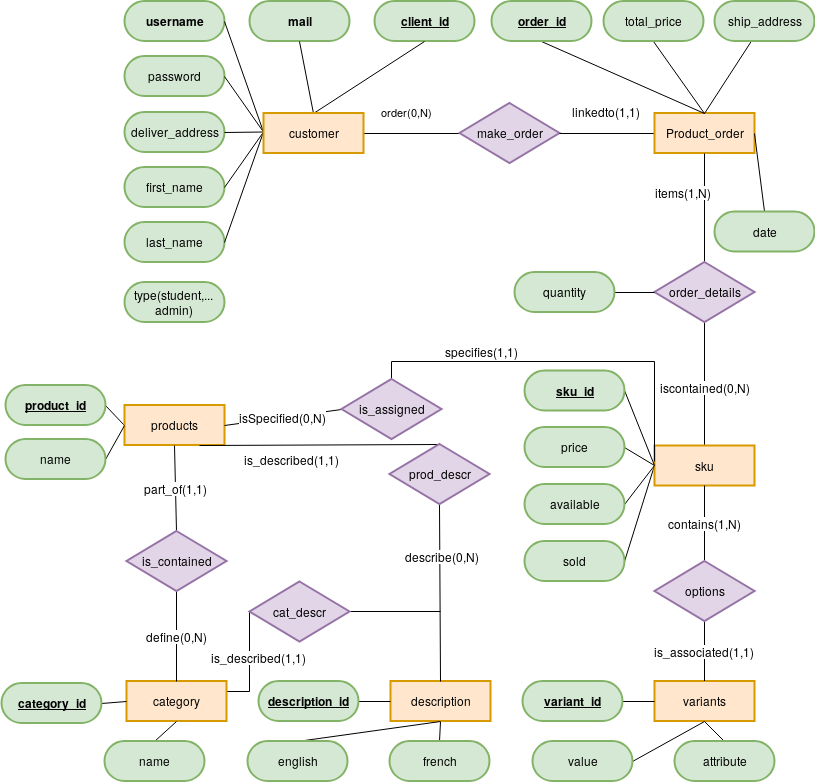
\includegraphics[scale=0.4]{./images/ecommerce_ER.png}
    \caption{eShop entity-relationship model}
    \label{ecommerce_er}
\end{figure}

\subsection{model to SQL tables}
The translation of the model depicted on \autoref{ecommerce_er} can be translated into SQL tables as \autoref{ecommerce_sql} shows.
\begin{figure}[h!]
    \centering
    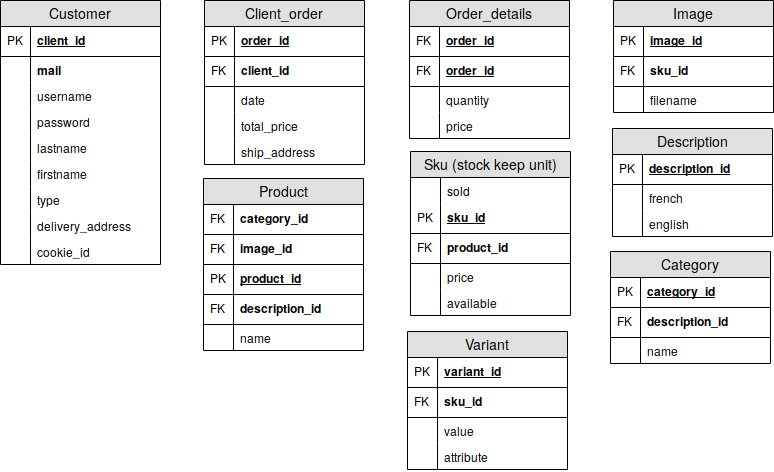
\includegraphics[scale=0.4]{./images/ecommerce_SQL.png}
    \caption{eShop entity-relationship model}
    \label{ecommerce_sql}
\end{figure}

\section{Website}
The website is divided into section. The first section is dedicated to the admin of the website itself an can only be accessed by users with the right privileges. The second second is dedicated to customer where they can buy products. For the development of the website we applied minimal protections like SQL injection and direct PHP scripts access protections.

\subsection{Admin panel}

\subsection{Customer View}

\subsubsection{Registration}
To purchase products, a customer needs to create an account on the website to do so, he needs to click on the button dedicated to that purpose or simply follow \textit{http://websitedomain.com/register.php}. On that page the user must fill fields with correct informations and then validate his account. If everything is correct he is redirected to the login page.
 
\subsubsection{Log in}
After the creation of an account a user can connect to the website by using his account informations. To achieve that he simply click on the button made for that purpose or going to \textit{http://websitedomain.com/login.php}. If the information given are correct he will be redirected on the home page.
 

\begin{figure}[h!]
    \centering
    \subfloat[register page]{{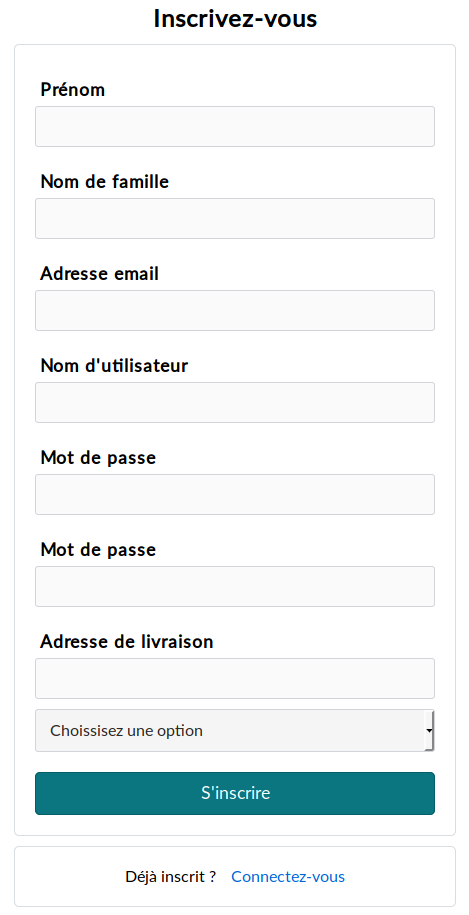
\includegraphics[scale=0.3]{./images/sign_up.png}}}%
    \qquad
    \subfloat[login page]{{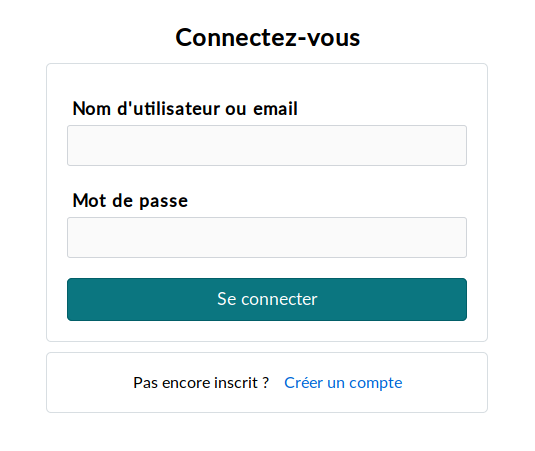
\includegraphics[scale=0.3]{./images/sign_in.png}}}%
    \caption{connection pages}%
    \label{fig:mineral}%
\end{figure}

The login page is the same for the admin, since the admin has more privileges when he is logged, he can access more pages such has the admin panel.
\end{document}

